
\section{Metabolic Response to Brain Activation} \label{sec:pain}

To further understand the origin of brain activation during the experience of pain and how this activity is modulated by the brain, a measure of brain activation is therefore needed. To get a measure of brain activation, the underlaying physiologic response is of great importance to understand. \\
The activation of a brain region starts with a neurological input containing information about the noxious stimuli \cite{Tracey2007}. The increased neurological activity affects local metabolism as processing of the signal requires adenosine triphosphate (ATP) consumption during e.g. the reception and reconstruction of the action potential. Thus, ATP starts to be processed, leading to a decrease in oxygen concentration and increase in waste products. Thereby, the metabolic need for oxygen increases. Subsequently, these changes occurring in the local tissue of the corresponding brain region activate a vasodilation, increasing the blood flow to that region to reestablish the local homeostasis. During this regulation a not yet fully understood phenomenon occurs, where more oxygenated blood than needed, to compensate for the offset, is delivered, which floods the local region with oxygenated blood. This response to the increased neural activity is known as the hemodynamic response. Thus, the hemodynamic response becomes an indirect measure of neural activity. \cite{Glover2011,Poldrack2011}  %The overall increase in neural activity in that specific region following the need for metabolic regulation thereby permits the measure of the hemodynamic response, hence becoming an indirect measure of the neural activity.
An example illustrating the hemodynamic response can se seen in \figref{fig:back:HRF}.

\begin{figure}[H]                 
	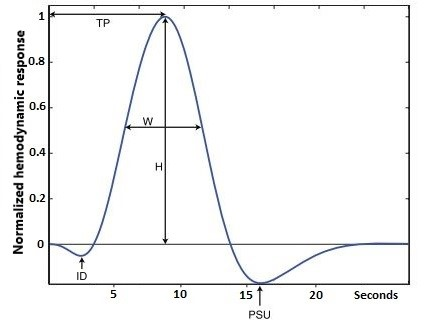
\includegraphics[width=.62\textwidth]{figures/aBackground/HRF}  
	\caption{A depiction of a single hemodynamic response curve. ID is the initial dip as less oxygen will be present as the metabolic demand increases, TP is time from stimulus until peak, W and H are the width and height of the response and PSU is a post stimulus undershoot. The illustration is adapted from \cite{Poldrack2011}.}
	\label{fig:back:HRF} 
\end{figure}

\Figref{fig:back:HRF} is a representation of a perfect noiseless hemodynamic response curve to a brief stimuli. However, in reality the response is affected by physiological noise and is delayed in time compared to the stimulus onset. The peak height of the curve is commonly the most interesting feature of the response, as it portrays the amount of neural activity the best. The time to peak will often occur 4-6 seconds after stimulus onset. The duration of a response is approximately 20 seconds. There will furthermore be a noticeable initial dip of 1-2 seconds duration, when the initial oxygen reserves are used up and a 20 second poststimulus undershoot as homeostasis is reestablished. \cite{Poldrack2011}   